\documentclass[a4paper]{article}
\usepackage{Graphicx}
\usepackage{fullpage}

\title{{RELACS: Reliable Estimator of Local Antagonizing and Counterproductive Sounds}}
\author{Steven Bosch \and Luuk Boulogne \and Pim van der Meulen \and Xeryus Stokkel  \and Rogier de Weert}

\begin{document}

\maketitle

\section{Product purpose}

\subsection{Problem}
Stress is arguably the biggest problem of our society nowadays. It can be very harmful to the health of the individual, as stress can cause problems in both mental and physical health. The effects of living a stressful life can include a reduced urge in reproduction, as well as lowered productivity during work. Throughout the years, many methods have been devised to decrease stress and increase relaxation. The system described onward does not decrease stress or increases relaxation directly, but rather attends the user to the influence of stress-inducing sounds in the environment of the user. When the user is more aware of stressful sounds in its sound environment (also called soundscape) he or she could change or avoid this environment, which might decrease their stress-level.

\subsection{Target group}
Since stress can be experienced by anyone, we did not feel like limiting our product to a specific target audience. We could say that our user group consists of students, people working in an office, construction workers, and the elderly. 
The current version of our product is aimed at an English-speaking audience, although in future versions we hope to increase our user-count with a wider selection of languages. 

\subsection{Improvements}
We aim to improve the user awareness of the stress-level in their surroundings.
By showing users that some of the sounds present in their environment are stress-inducing, we want to improve the awareness of the importance of sound in order to create or find a relaxed environment. 
We think that a relaxed environment would benefit a person, as productivity is higher when stress is lower.

\section{Product description}
In the next chapter the complete technical specifications can be found, followed by a performance analysis and a user manual. 
But first a simple representation of the working of RELACS is given. RELACS is a simple tool to see how stressful a sound-sample is. 
When a processed recording of 30 seconds is presented to the tool, it calculates the overall percentage of stressfulness of the sample and shows where in the sample the stressful sounds are located. 
Basically what RELACS does is: sound in, stress analysis out.

A processed recording means that a recording (.wav-file) should first be processed to a cochleogram (as in a .hdf5 file) before it can be presented to RELACS. The system then cuts the sample in windows of each 128

\section{Technical specifications}


\section{Performance analysis}

\subsection{Strengths}
\subsection{Weaknesses}
\subsection{Opportunities}
\subsection{Threats}


\section{User manual}
Currently RELACS only works web-based and with .hdf5 files as input. At the homepage a list of previous analyses can be found, with their respective stressful-percentage. This can be used to compare samples taken at a specific place, bt at a different time. The names of each 



\section{Pitch sheets}

\begin{figure*}[h]
\centering

\includegraphics[width=\linewidth]{./Slide1}
\label{fig:Slide1}
\end{figure*}

\begin{figure*}[h]
\centering
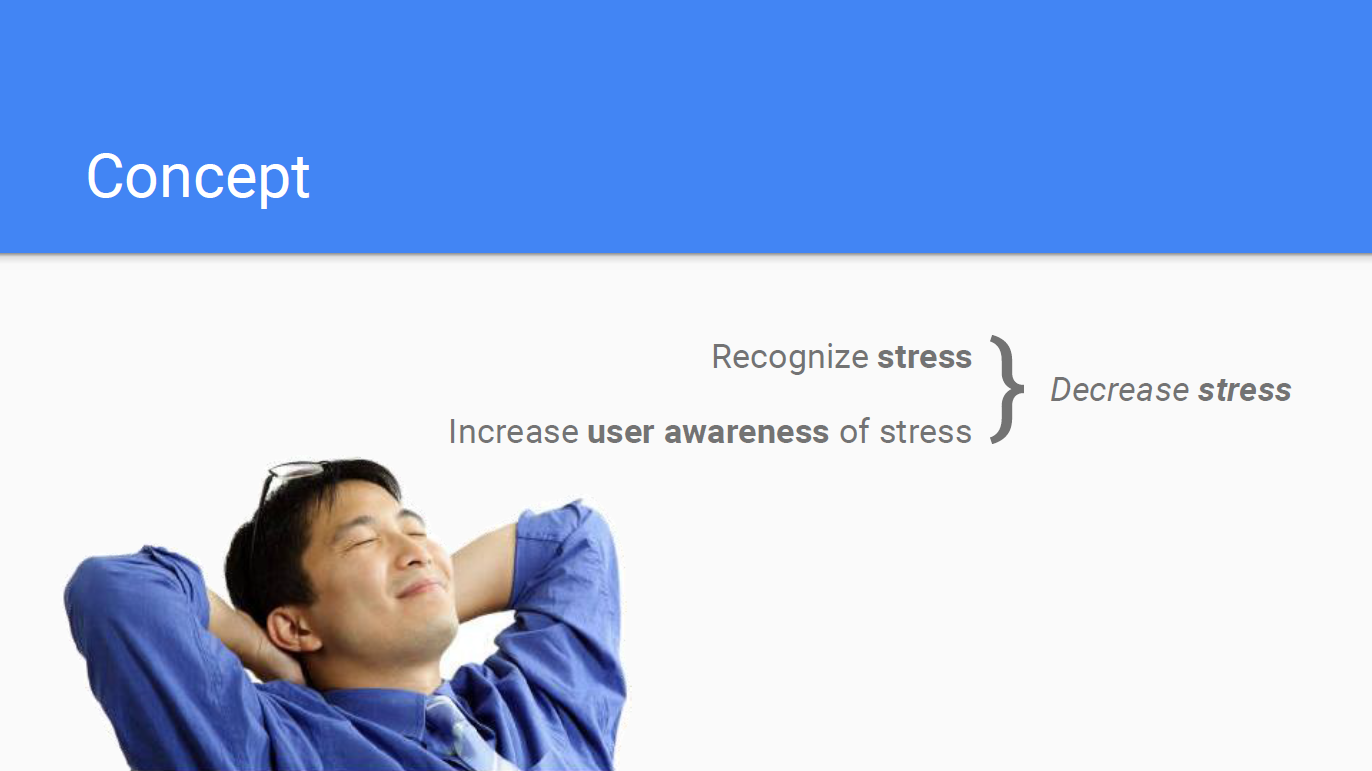
\includegraphics[width=\linewidth]{./Slide2}
\label{fig:Slide2}
\end{figure*}

\begin{figure*}[h]
\centering
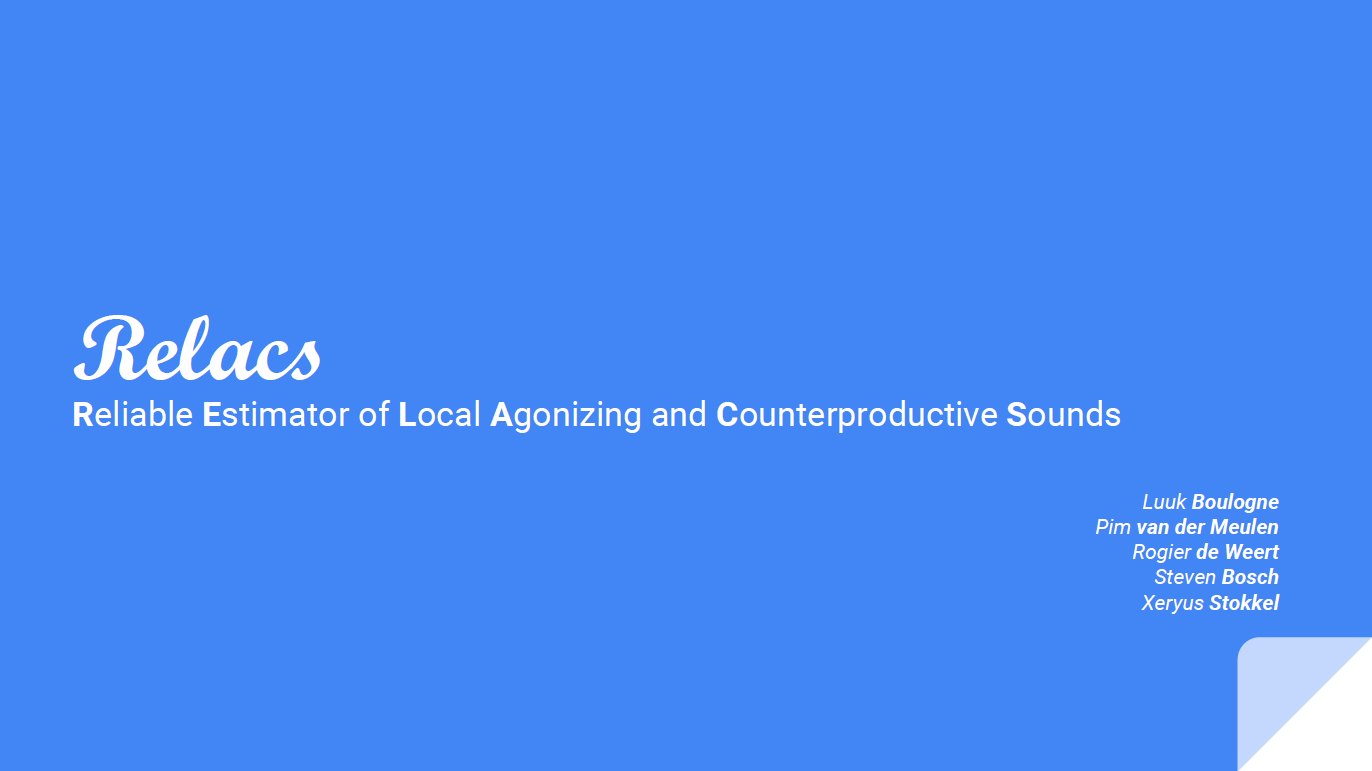
\includegraphics[width=\linewidth]{./Slide3}
\label{fig:Slide3}
\end{figure*}

\begin{figure*}[h]
\centering
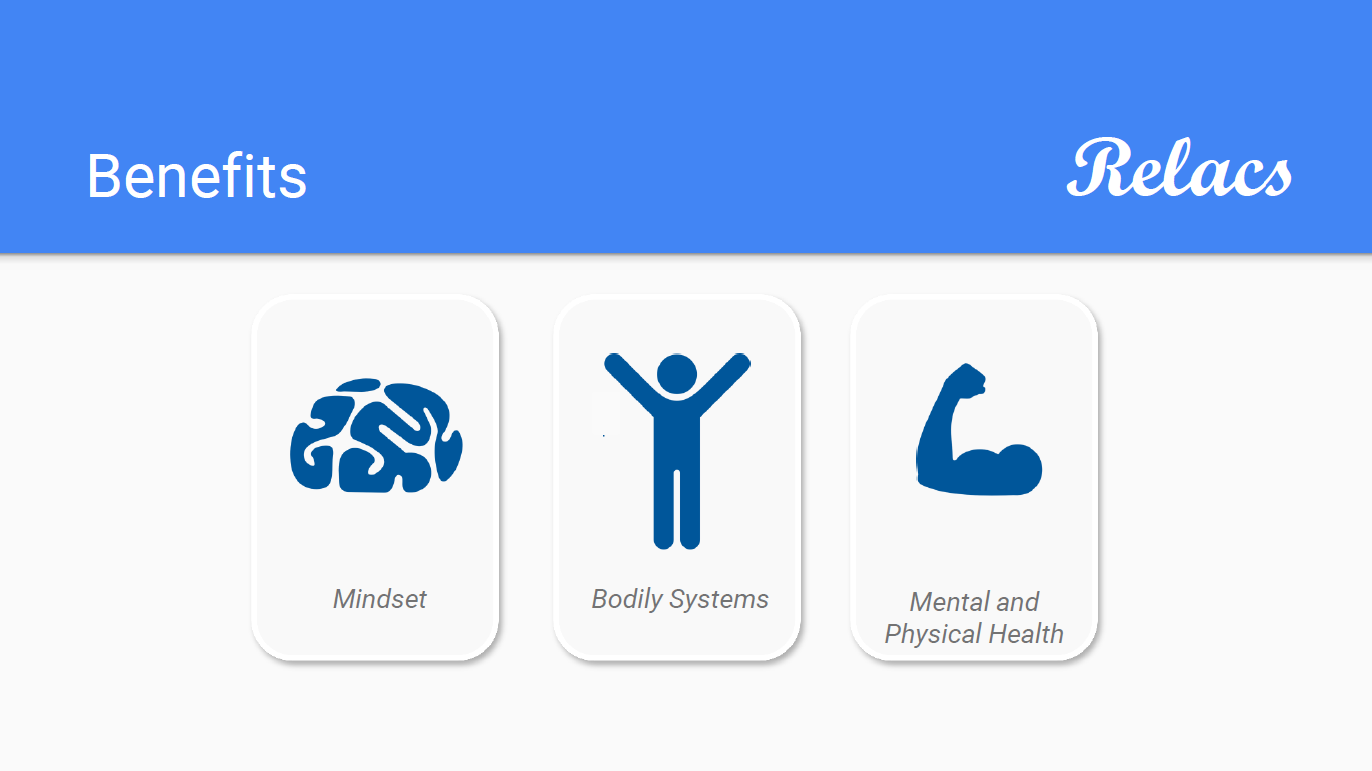
\includegraphics[width=\linewidth]{./Slide4}
\label{fig:Slide4}
\end{figure*}

\begin{figure*}[h]
\centering
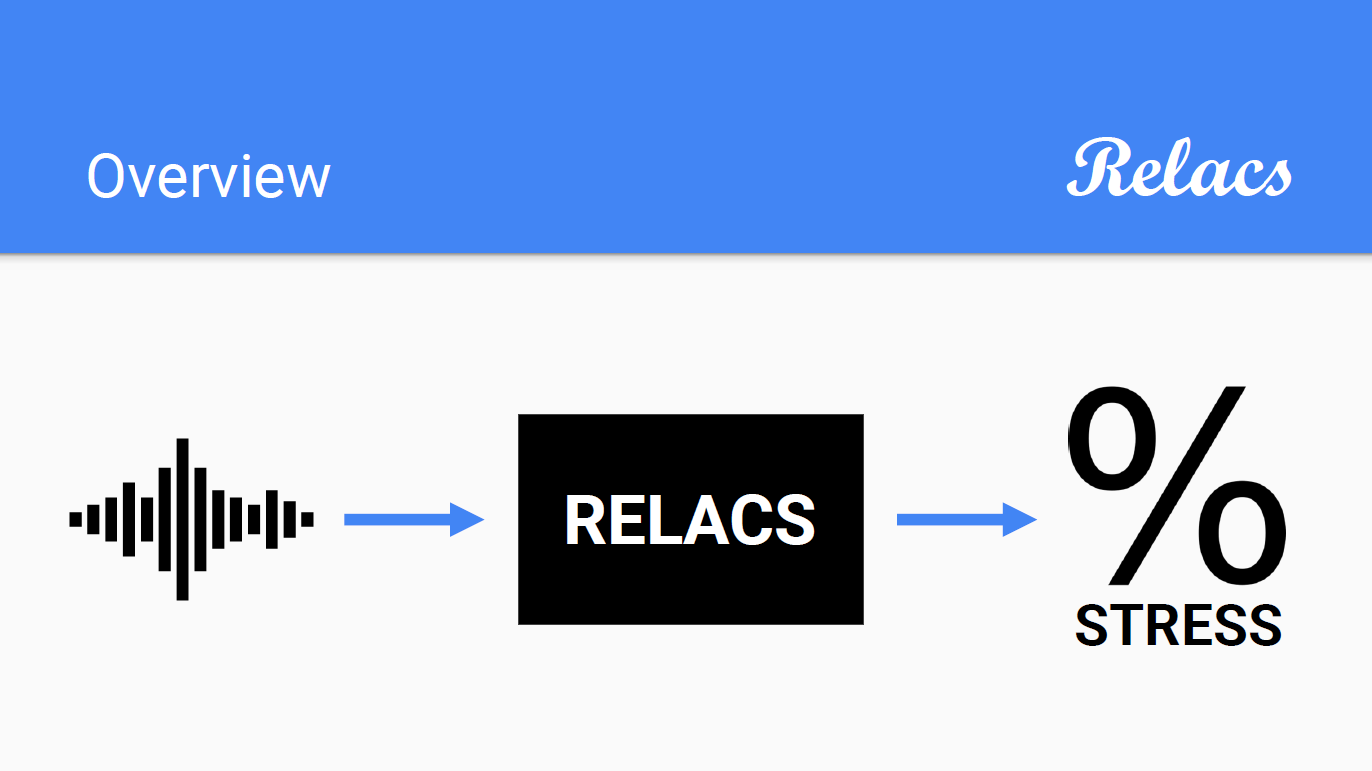
\includegraphics[width=\linewidth]{./Slide5}
\label{fig:Slide5}
\end{figure*}

\begin{figure*}[h]
\centering
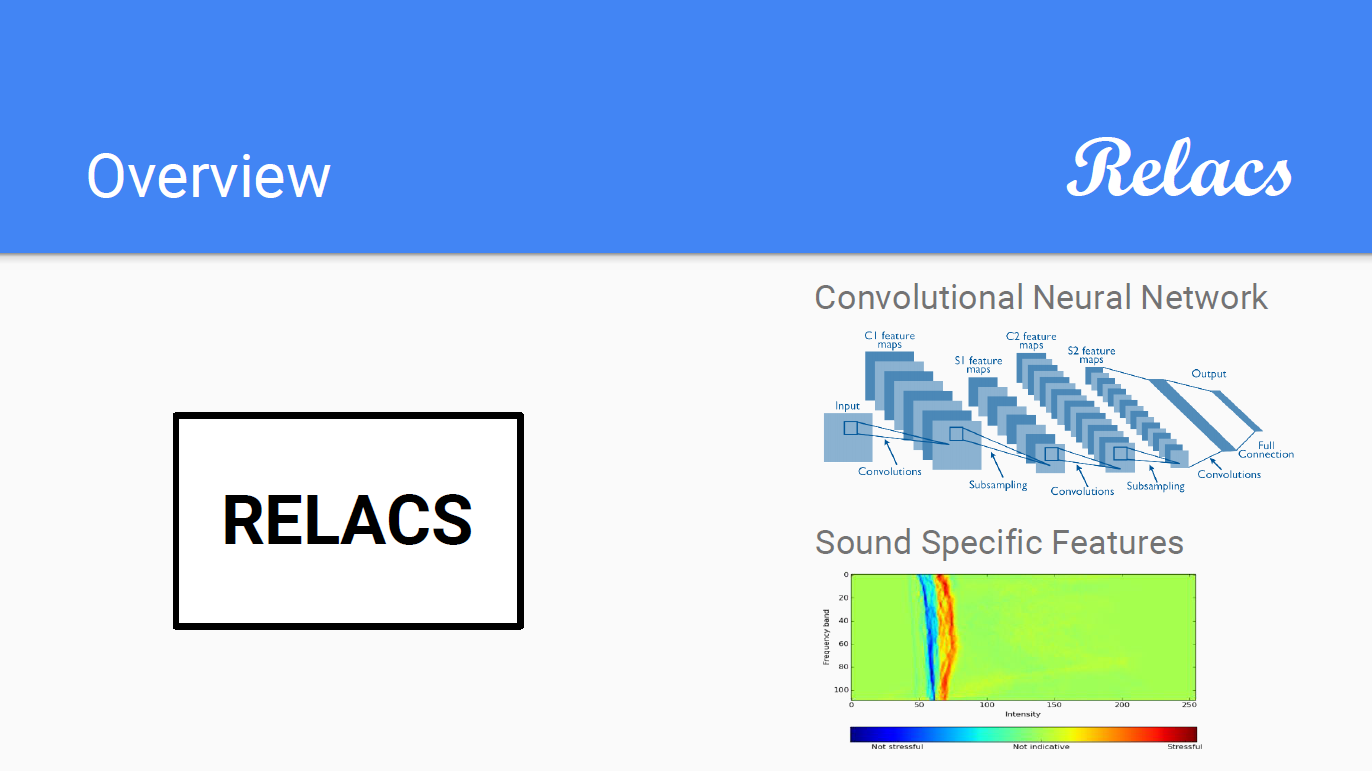
\includegraphics[width=\linewidth]{./Slide6}
\label{fig:Slide6}
\end{figure*}

\begin{figure*}[h]
\centering
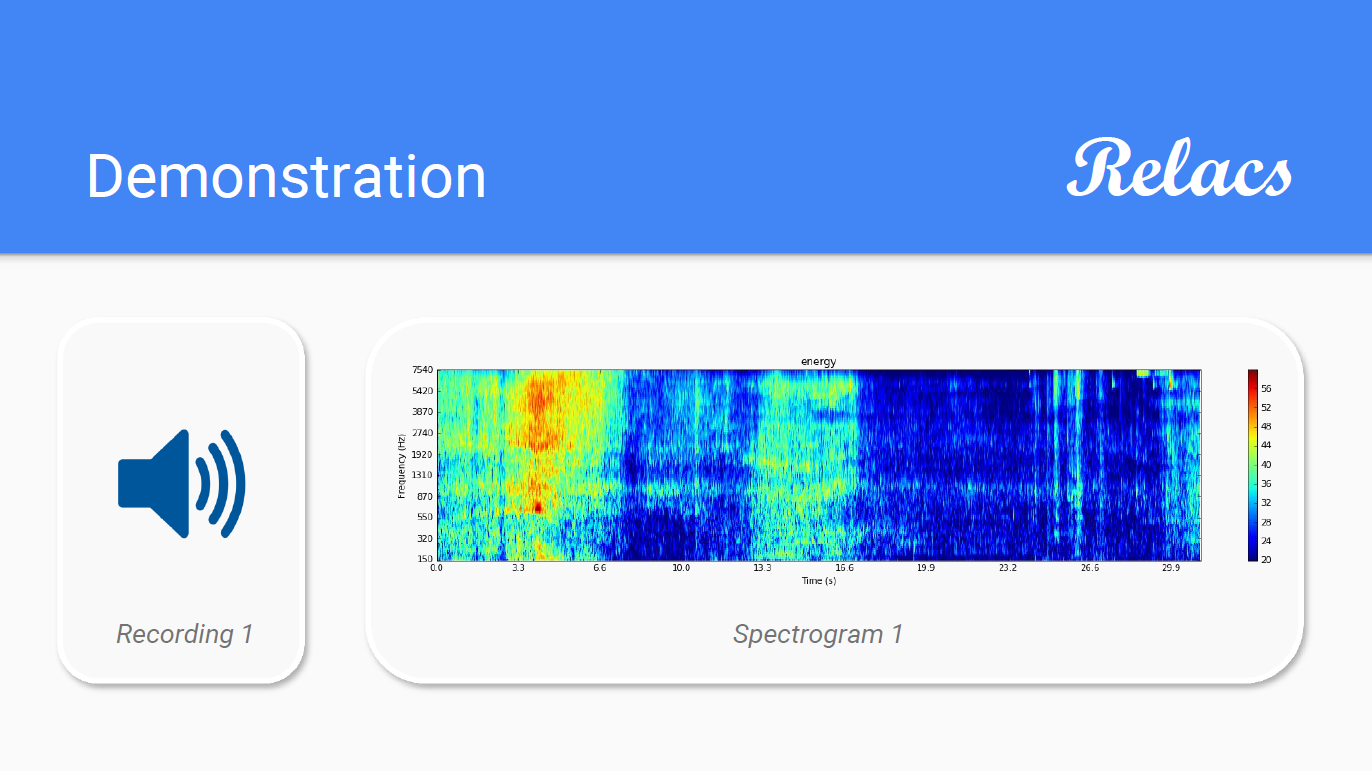
\includegraphics[width=\linewidth]{./Slide7}
\label{fig:Slide7}
\end{figure*}

\begin{figure*}[h]
\centering
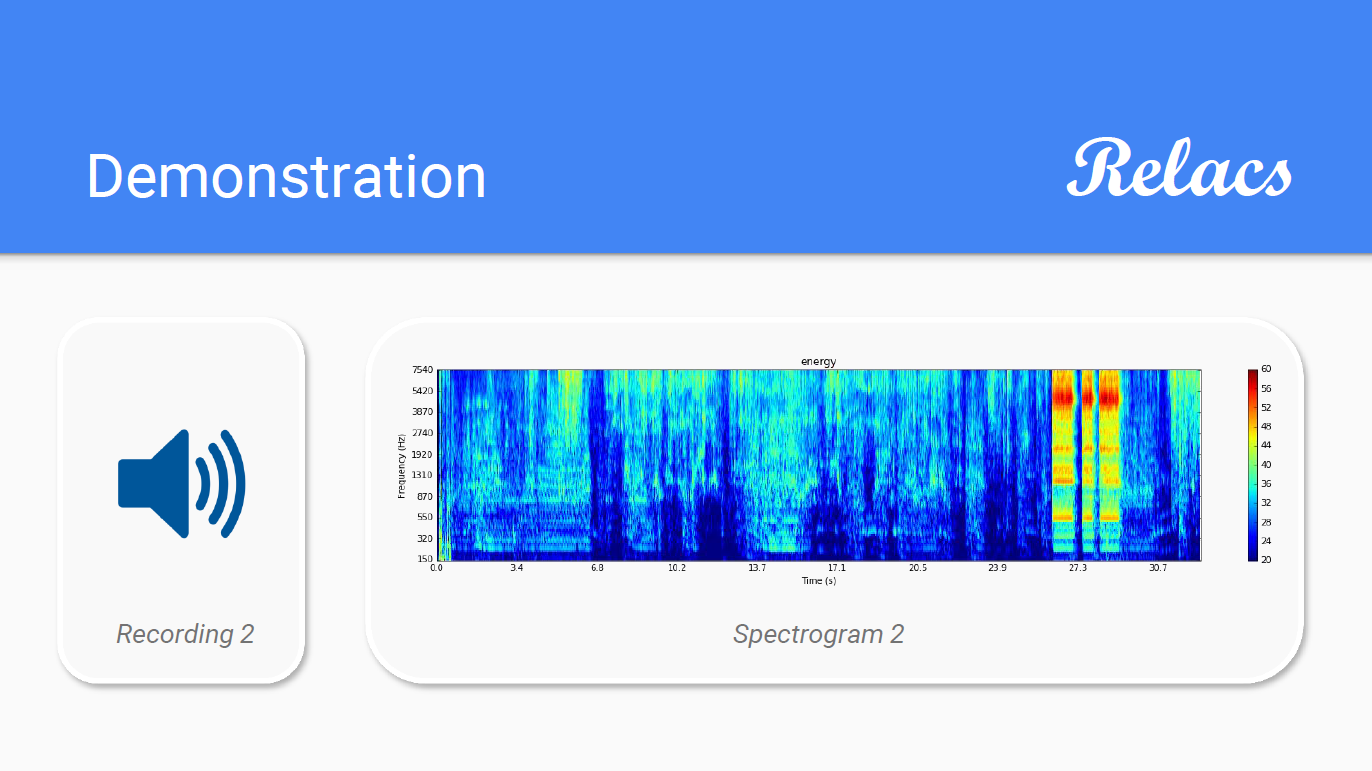
\includegraphics[width=\linewidth]{./Slide8}
\label{fig:Slide8}
\end{figure*}

\begin{figure*}[h]
\centering
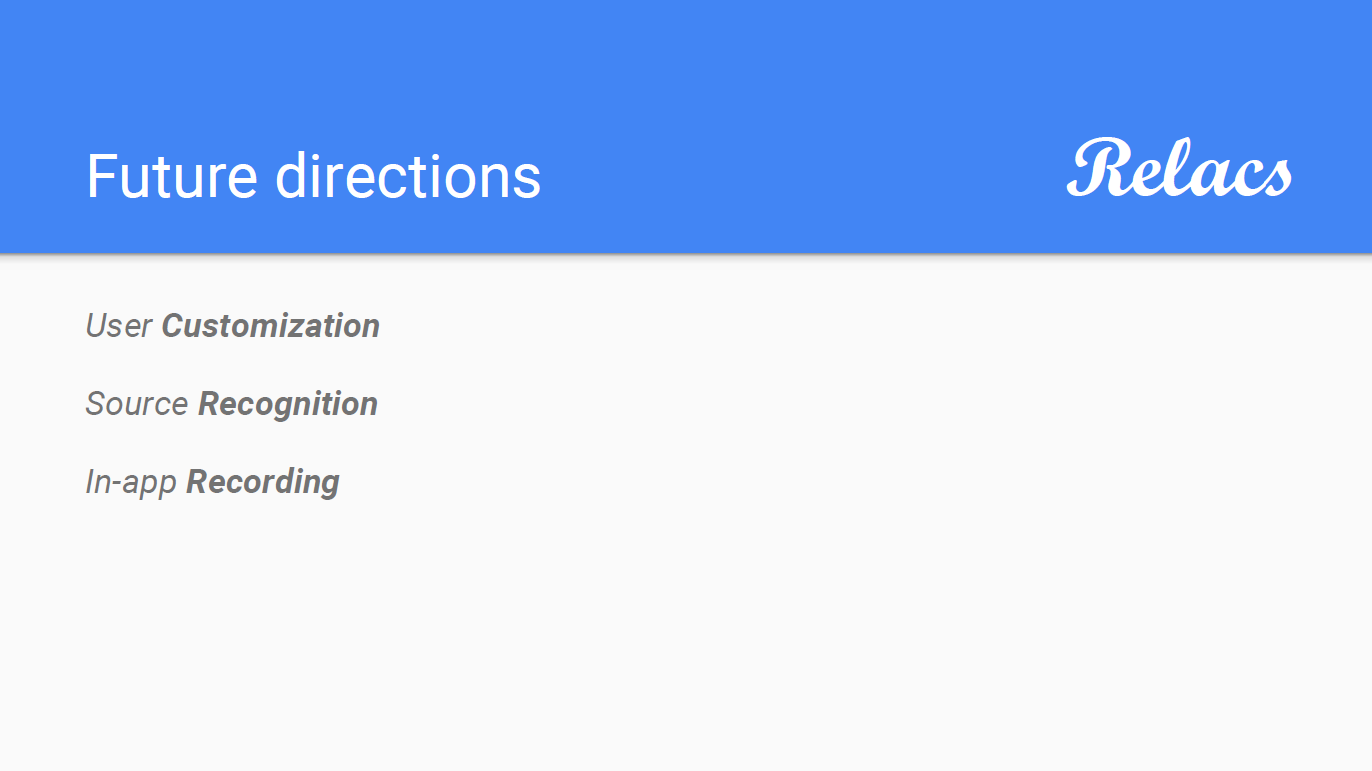
\includegraphics[width=\linewidth]{./Slide9}
\label{fig:Slide9}
\end{figure*}

\end{document}
